%!TEX root = cscw2018-comic.tex

\section{Results}
\label{sec:Results}

\subsection{Raw Data}
\label{sub:Raw Data}
In total we have 146 participants joined our study, 73 of them in negative framed condition and 73 of them in positive framed condition. 5 participants are removed due to incomplete data. 4 participants are removed due to failed at least one attention check question. 6 participants are removed due to multiple attempts. The following analysis is based on a dataset with 131 participants (655 observations), 63 of them is in positive framed condition and 68 of them in negative framed condition.

\subsection{Bayesian Model}
\label{sub:Bayesian Model}
We use a Bayesian formulation of the problem of identifying suitable predictors for the messages in comic form.~\textcite{Kay2016} provide an nice introduction on the appropriateness of Bayesian analysis for the HCI community. Bayesian analysis is attractive in our experiment due to two advantages: shifting the conversation from ``did it work'' to ``how strong is the effect''; and benefits to small $n$ studies.

We manipulate five independent variables: gesture of the participants in the comic (3: neutral, moderate, extreme);  distance between the two characters (3:close, moderate, far); comic shading (3:white, light gray, gray); framing (2: whether the information was positively framed or negatively framed).  This gives us a total of $3 \times 3 \times 3 \times 2= 54$ experimental conditions. As a control against ordering effects, we randomly manipulate comic position (whether we presented the comic panel to the left or to the right).  Thus, we need to estimate the effect on the responses for each of these variables; the responses are on a 7 point Licket scale.

A challenge with using ordinal scale such as the Lickert scale: we do not know the ``width'' of each response. That is, while we may know that for example $1<2<3$, we don't know if the difference in the thresholds used by subjects to mark ``2'' on the scale, is the same as the difference in thresholds they use for ``1'' and ``3.''  We assume that each response by a subject: lies in a continuous metric space; is Normally distributed; and that the thresholds $\{\theta_i\}$ while unknown, are shared—all subjects use same set of thresholds to identify the appropriate ordinal value.

Formally let $z$ be the response of the subjects to the experiment where the comic panel was generated by the different conditions; each condition is obtained by setting each of the $k$ independent variables $\{x_j\}, j \in [1 \ldots k]$. The subjects first generate a Normally distributed metric variable $y$, and then use the thresholds $\{\theta_i\}$ to map $y$ to the ordinal variable $z$.

Then, since we assume that the metric variable $y$ is Normally distributed, our hierarchical Bayesian model is defined as follows (see~\Cref{fig:generative-main} for a graphical representation):

\begin{align}
 y                  & \sim N(\mu, \sigma_y)                    \label{eq:response-main}                       \\
 \sigma_y           & \sim U(L, H), \label{eq:main-sigma}                                                     \\
 \mu                & \sim \beta_0 +
 \underbrace{\sum_{j} \beta_{1,j} x_{1,j}(i)}_{\text{gesture}} +
 \underbrace{\sum_k \beta_{2,k} x_{1,k}(i)}_{\text{shading}} +
 \underbrace{\sum_l \beta_{3,l} x_{1,l}(i)}_{\text{distance}} +
 \underbrace{\sum_m \beta_{4,m} x_{1,m}(i)}_{\text{framing}} ,                  \label{eq:mu-main} \\
 \sum_j \beta_{i,j} & = 0, \qquad  \qquad  \quad \, i \in \{1, \ldots, 4\}, \label{eq:beta-equality}          \\
 \beta_{i,j}        & \sim N(0, \sigma_{\beta, i}), \qquad  i \in \{1, \ldots, 4\},\label{eq:main-beta-sigma} \\
 \sigma_{\beta, i}  & \sim \Gamma(s, r ). \label{eq:gamma-distribution}
\end{align}
\Cref{eq:response-main} says that the metric variable $y$ is Normally distributed\footnote{The ``$\sim$'' symbol means that the random variable on the left is drawn from the probability distribution on the right.} with mean $\mu$ and standard deviation $\sigma_y$.~\Cref{eq:mu-main} says that the mean response $\mu$ is a linear weighted combination of the predictors.~\Cref{eq:main-sigma} says that the standard deviation of the response is drawn from a Uniform distribution with constant parameters $\text{Low}=L, \text{High}=H$, where $L>0, H\gg L$.~\Cref{eq:main-beta-sigma} says that the predictor weight is drawn from a Normal distribution with $\mu=0$ and standard deviation $\sigma_{\beta, i}$. That is,  while \textit{each} predictor set $\beta_{i}$ is drawn from a \textit{different} Normal distribution, the $\beta_{i,j}$ values within the same predictor set $\beta_{i}$ are drawn from the \textit{same} Normal distribution.~\Cref{eq:beta-equality} says that the sum of the deflections $\sum_k \beta_{j,k}$ from the mean for any nominal predictor $j$ equals zero.~\Cref{eq:gamma-distribution} says that we draw all the variances $\sigma_{\beta, i}$ from a Gamma $\Gamma(s,r)$ distribution, where $s$ refers to the shape parameter and $r$ refers to the rate parameter. We set the variables $s,r$ to allows a wide range of values for $\sigma_{\beta, i}$.

By drawing the standard deviation variables $\sigma_{\beta, i}$ from a Gamma distribution, the values of each element of $\beta_i$ informs the other elements. Notice that we draw the variances $\sigma_{\beta, i}$ of each predictor $i$ from an independent Gamma distribution, implying that the variances (equivalently, the extent of deflections from the mean) for each predictor can be different. Furthermore, the ``information sharing'' among variables is common to hierarchical Bayesian models and is an important reason why Bayesian models work so well with small datasets\footnote{The sharing of information causes the variance of each individual element $\beta_{i,j}$ to move towards the group variance, a phenomena known as ``shrinkage.'' }. The main advantage of using a Gamma distribution is that we can specify a non-zero mode, important in controlling shrinkage in hierarchical models.

\begin{figure}
 \centering
 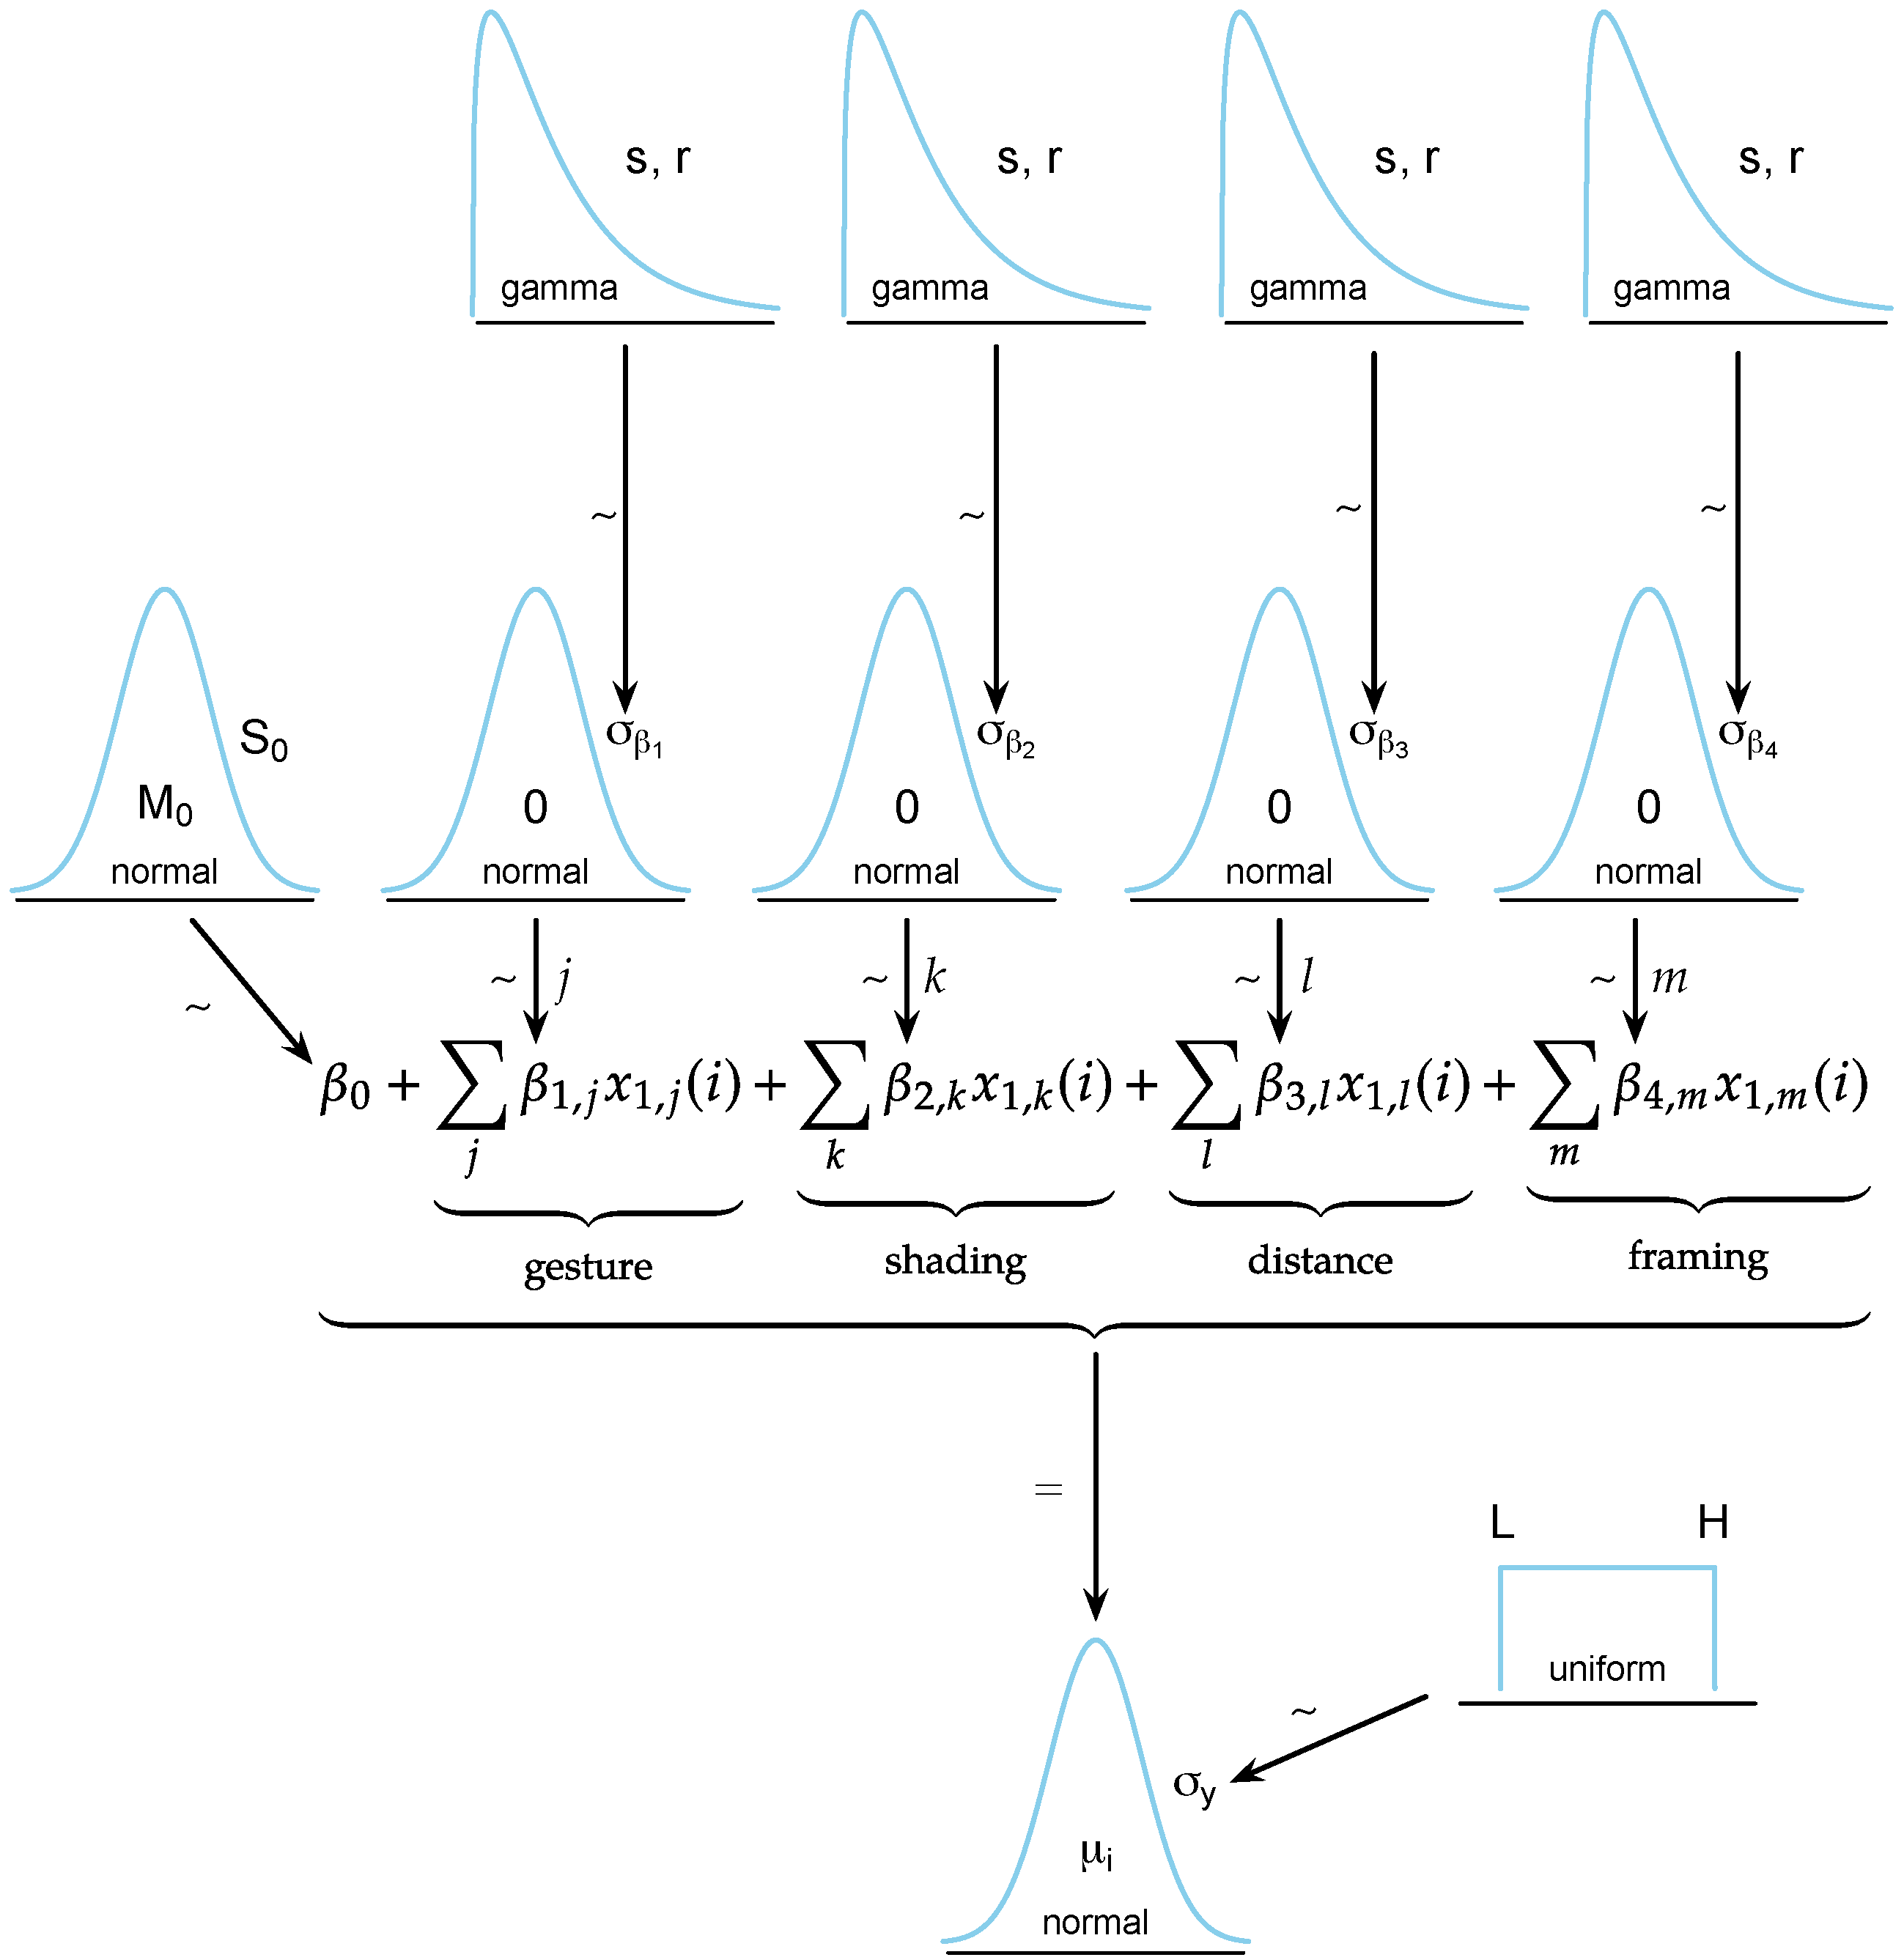
\includegraphics[width=0.67\textwidth]{./figures/generative_model.pdf}
 \caption{The figure shows the hierarchical Bayesian model specification, corresponding to~\Crefrange{eq:response-main}{eq:gamma-distribution}.}
 \label{fig:generative-main}
\end{figure}

Thus far, we have discussed how to generate a Normally distributed metric variable $y$. However, what we see in the experiment is not this metric variable, but an ordinal variable $r$. The subjects use internal thresholds $\{\theta_i\}$ to determine when to ``strongly disagree'', ``disagree'' etc. Thus with a 7 point Likert scale, we have 6 thresholds. The probability that we will see an ordinal response $r=k$ is $P(r=k | \mu, \sigma, \{\theta_i\})$, where, $\{\theta_i\}$ is the set of thresholds used by the subjects. We assume that while these thresholds are unknown, all subjects use the same thresholds. Since the underlying metric response $y$ is Normally distributed, we can compute the probabilities for observing each ordinal response $r=k$ as follows:

\begin{equation}
 P(r=k | \mu, \sigma, \{\theta_i\}) = \Phi \left (\frac{\theta_k - \mu}{\sigma} \right) - \Phi \left(\frac{\theta_{k-1} - \mu}{\sigma} \right).
\end{equation}
Where, $\Phi$ represents the cumulative density function for the Normal distribution corresponding to the underlying metric variable $y$. In other words, the probability that we will see ordinal response $k$ is the area under the Normal distribution with parameters $\mu, \sigma$ between thresholds $\theta_{k-1}$ and $\theta_k$.

The thresholds $\theta_i, i \in \{2, 3, 4, 5\}$ have two degrees of freedom in that a simple translation of the response will translate the thresholds. Consistent with~\textcite[][p. 674]{Kruschke2014}, we set $\theta_1\equiv1.5$ and $\theta_6\equiv6.5$, leaving us with four hidden threshold parameters. We draw these remaining four $\{ \theta_i\}$ from a Normal distribution as follows:
\begin{equation}
 \theta_i \sim N(i+0.5, 1/2), i \in \{2, 3, 4, 5\}.
\end{equation}

In this section, we developed a hierarchical Bayesian formulation to model the subject ordinal response to analyze the effect of different predictors for three comic elements (gesture, distance, shading) and information framing. We have a total of $54$ experimental conditions. We also modeled the thresholds for the different ordinal outcomes as a hidden variable. In the next section, we present and analyze the results.

\subsection{Analysis}
\label{sub:Analysis}

We analyzed the data using PyMC3~\cite{Salvatier2016}, a popular framework for Bayesian inference. Computational techniques for Bayesian inference use a stochastic sampling technique called Markov Chain Monte Carlo (MCMC) that samples the posterior distribution $P(\theta | D)$, where we want to estimate the parameters $\theta$ given the observations $D$. In particular, we used the Metropolis-Hastings sampler. The Gelman-Rubin statistic $\hat{R}$ was around 1, indicating that the different sampling chains converged. The modal values of the coefficients are shown in~\Cref{tab:modal values}.:

\begin{table}[htb]%\footnotesize
 \centering
 \caption{Modal coefficient values $\beta_{0-4}$. Some coefficients are vectors as they represent the displacement from the mean for different conditions of that variable. For example, since gesture has three experimental conditions, $\beta_1$ is a vector of length 3.}\label{tab:modal values}
 \begin{tabular}{@{}rl@{}} \toprule
  Coefficient                                       & Values                     \\ \midrule
  Intercept ($\beta_0$)                             & $4.524$                    \\
  Gesture: [Neutral, Medium, Extreme] ($\beta_1$)   & $[-0.218, 0.101, 0.118]$   \\
  Shading: [Neutral, Light Gray, Gray] ($\beta_2$)  & $ [-0.218 , 0.101, 0.118]$ \\
  Distance: [Closest, Medium, Farthest] ($\beta_3$) & $[-0.043, -0.057, 0.099]$  \\
  Framing: [Negative, Positive] ($\beta_4$)         & $[ 0.051, -0.051]$         \\
  Standard Deviation ($\sigma_y$)                   & $1.614$                    \\ \bottomrule
 \end{tabular}
\end{table}


\Cref{fig:main-experiment-effect} shows the mean effect and the effect size, as well as the contrast between positive and negative messages. The mean effect has a mode at $\mu=4.53$ with the High Posterior Density (HPD\footnote{The HPD interval is the location of 95\% of the posterior density. This is similar to, but different from the idea of confidence interval used in classical statistics. See~\textcite{Hoekstra2014} for a discussion on the misinterpretation of confidence intervals.}) interval of $[4.35, 4.70]$. Since the HPD lies outside a meaningful ROPE (Region of Practical Equivalence)\footnote{Unlike classical statistics, where one can ask for example, if the two means for two treatments are different $P(\mu_1\neq \mu_2)$, in Bayesian statistics, one asks if the HPD interval of the distribution $P(\mu_1-\mu_2)$, the difference of the means of the two treatments, excludes an interval where we can consider the two treatments equivalent. This equivalence interval is domain dependent. In the Lickert scale, one could argue that $[4 \pm 0.25]$, is a meaningful ROPE for the mean effect, since the neutral effect case is $\mu=4$, although smaller ROPEs of $[4 \pm 0.1]$ are also used.} of $4 \pm 0.25$, the result implies that there is a clear effect due to the treatment. Furthermore, the figure shows a moderate effect size of $0.33$; we consider an effect of $0.2$ to be small, and an effect of $0.5$ is a medium sized effect. Since the distribution excludes the ROPE interval $[0 \pm 0.1]$, the discovered effect size is significant.


~\Cref{subfig-2:framing} shows the contrasts between a negatively framed message and that of a positively framed message. The figure shows that a negatively framed message seems to have more of an effect, but since the distribution includes a ROPE of $0 \pm 0.1$, the effect is not significant. Slightly more than $80\%$ of the posterior lies beyond 0, suggesting that effects of a negatively framed message may be more clear in a larger study.



\begin{figure}
 \subfloat[The mean effect and the effect size\label{subfig-1:mean-effect}]{%
  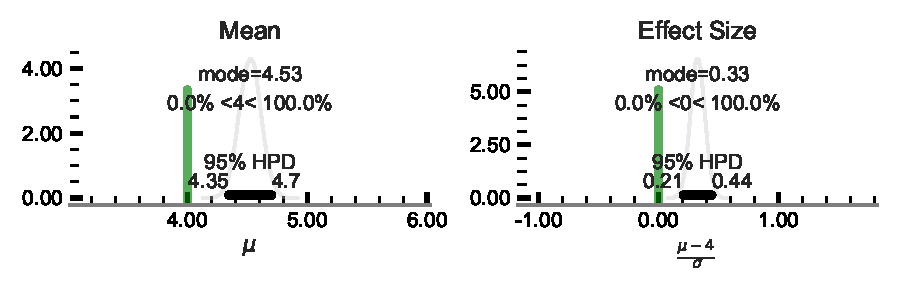
\includegraphics[width=0.6\textwidth]{./hari-code/factors_mean_effect_main-noint.pdf}
  } \hfill
 \subfloat[Information framing contrast\label{subfig-2:framing}]{%
  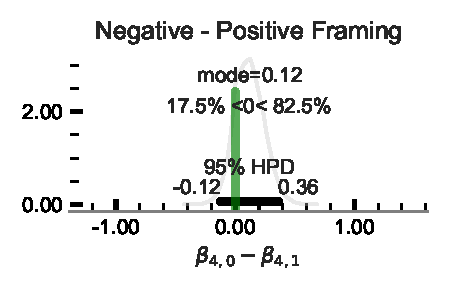
\includegraphics[width=0.33\textwidth]{./hari-code/factors_framing_contrasts_main-noint.pdf}
 }
 \caption{~\Cref{subfig-1:mean-effect} shows the High Posterior Density (HPD) intervals for the mean response $\mu$ and effect sizes $\sigma_y$. HPD represent the region with 95\% of the density. Notice that the HPD interval for $\mu$ is $[4.35, 4.70]$ and excludes a ROPE of $[4\pm 0.1]$ (the interval includes 4, the neutral response value), implying that on average, the response to the comic panel was more persuasive than the text. The figure for effect size shows a moderate effect with mode $0.33$; since the HPD interval $[0.21, 0.44]$ excludes a ROPE of $[0\pm 0.1]$, we can be confident about the effect.~\Cref{subfig-2:framing} shows the contrasts between negatively framed message with a positively framed message. The modal value is $0.10$, but since the HPD interval $[-0.13, 0.36]$ overlaps with 0, there is no appreciable effect (but notice that 80\% of the density lies in the region greater than 0.)}
 \label{fig:main-experiment-effect}
\end{figure}

~\Cref{fig:theta-main} shows the posterior distribution of the thresholds $\{\theta_i\}$. We notice that the distributions for $\theta_2, \theta_3, \theta_5$ are outside  ROPE intervals $2.5 \pm 0.1, 3.5 \pm 0.1, 5.5 \pm 0.1$, implying that the discovered thresholds are significant.

\begin{figure}
 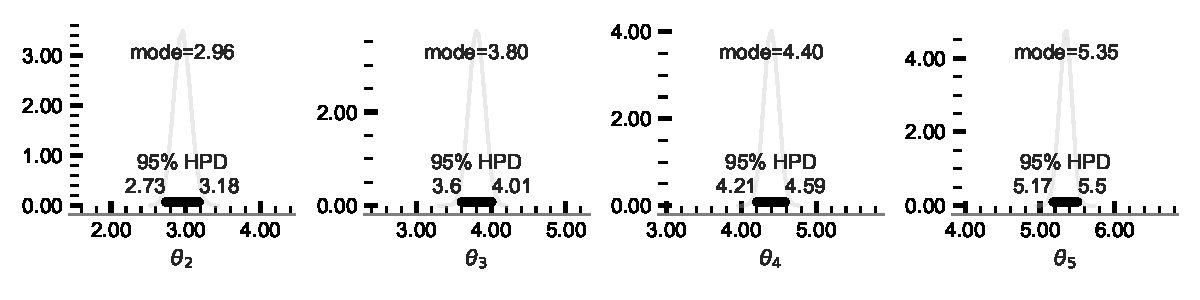
\includegraphics[width=\textwidth]{./hari-code/factors_theta_values_main-noint.pdf}
 \caption{The figures show the posterior densities of the different values of $\{\theta_i\}$, the thresholds estimated from the data. Notice that while the modal values are all different from the ideal cases $\{2.5, 3.5, 4.5, 5.5\}$, the posterior for $\theta_2$ is outside the ROPE of $[2.5\pm 0.1]$, and the posterior densities for $\theta_3$ and $\theta_5$ are just outside the corresponding ROPEs of $[3.5 \pm 0.1]$ and $[5.5 \pm 0.1]$.}
 \label{fig:theta-main}
\end{figure}

~\Crefrange{fig:gesture-contrasts-main}{fig:distance-contrasts-main}, show contrasts due to gesture, shading and distance. The results shown in~\Cref{fig:gesture-contrasts-main} indicate that while there is no significant difference between the gestures (all posteriors include a rope of $[0 \pm 0.1]$ ) a change from the neutral gesture has strong effect (more than 96\% of the posterior excludes 0), but that extreme and medium gesture show almost no difference. The results shown in~\Cref{fig:shading-contrasts-main} indicate that while there  is no significant difference between the gestures (all posteriors include a rope of $[0 \pm 0.1]$ ), a change from a neutral white background produces a strong effect (more than 97\% of the posterior excludes 0), but there is no discernible difference between light gray and gray background color.~\Cref{fig:distance-contrasts-main} shows that while there  is no significant difference between the distance conditions (all posteriors include a rope of $[0 \pm 0.1]$ ), a change to the farthest distance between the comic characters produces a moderate effect (more than 83\% of the posterior excludes 0); there is no discernible difference between the closest and the medium distance conditions.

\begin{figure}
 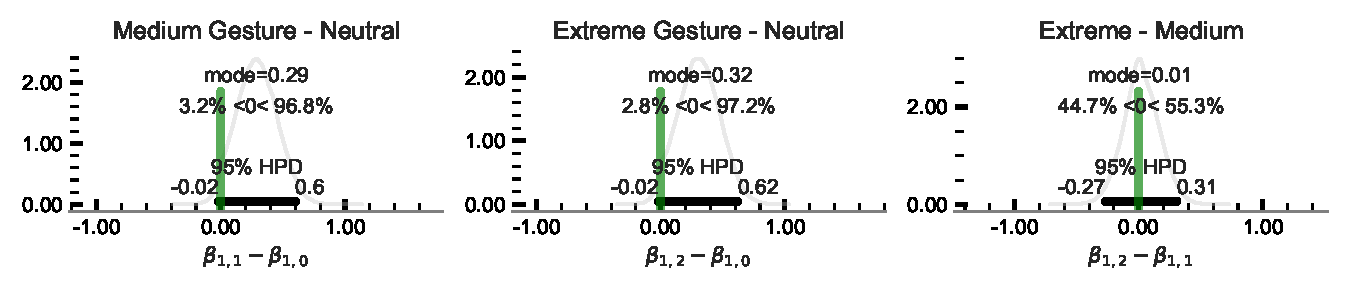
\includegraphics[width=\textwidth]{./hari-code/factors_gesture_contrasts_main-noint.pdf}
 \caption{The figure shows the contrast distribution for gestures; that is, it shows the distribution of $\beta_{1,i} - \beta_{1,j}$, where $i$ and $j$ are two different gesture conditions. The figures show that no difference distribution excludes $0$, hence none of the differences are significant. Both ``Medium'' and ``Extreme'' gestures have stronger effects on the preference towards comic when compared to ``Neutral'' (more than 96\% of the density is greater than 0); There is little difference between ``Extreme'' and ``Medium'' gestures. The result suggests that anything other than a neutral gesture is makes the comic panel more salient.}
 \label{fig:gesture-contrasts-main}
\end{figure}

\begin{figure}
 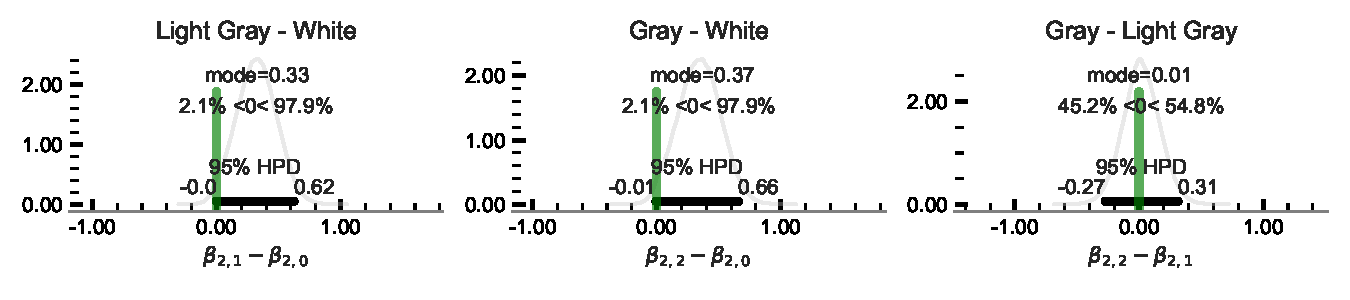
\includegraphics[width=\textwidth]{./hari-code/factors_shading_contrasts_main-noint.pdf}
 \caption{The figure shows the contrast distribution for shading; that is, it shows the distribution of $\beta_{2,i} - \beta_{2,j}$, where $i$ and $j$ are two different gesture conditions. The figures show that no difference distribution excludes $0$, hence none of the differences are significant. Both ``Light Gray'' and ``Gray'' shading have stronger effects on the preference towards comic when compared to ``White'' (more than 97\% of the density is greater than 0); There is little difference between ``Light Gray'' and ``Gray.'' The result suggests that anything other than neutral makes the comic message salient.}
 \label{fig:shading-contrasts-main}
\end{figure}

\begin{figure}
 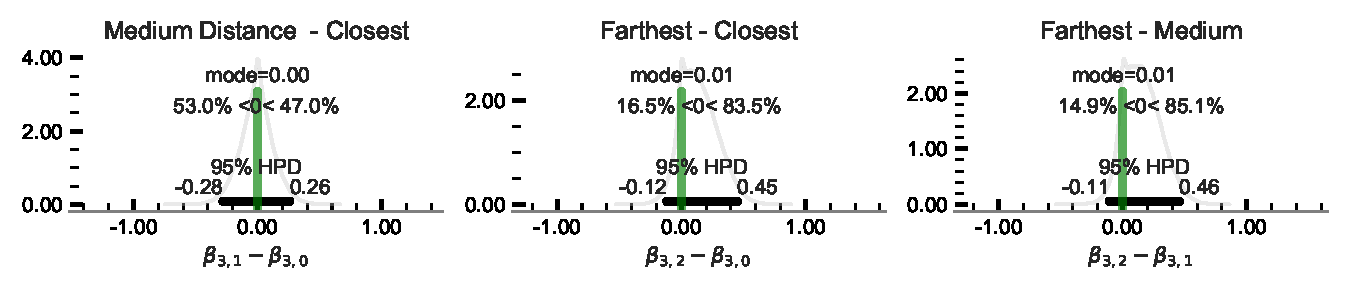
\includegraphics[width=\textwidth]{./hari-code/factors_distance_contrasts_main-noint.pdf}
 \caption{The figure shows the contrast distribution for distance; that is, it shows the distribution of $\beta_{3,i} - \beta_{3,j}$, where $i$ and $j$ are two different distance conditions. The figures show that no difference distribution excludes $0$, hence none of the differences are significant. Both ``Farthest'' shading have stronger effects on the preference towards comic when compared to ``Closest''  or ``Medium'' (more than 83\% of the density is greater than 0); There is little difference between ``Closest'' and ``Medium.'' The result suggests that extreme distances between are needed for them to be salient in the comic.}
 \label{fig:distance-contrasts-main}
\end{figure}

In this section, we presented a hierarchical Bayesian model to analyze the overall effect of using a comic to communicate facts, and understand the effect of three comic elements (gesture, shading and distance) and that of information framing. The results show that the use of comic produces a significant effect ($\mu=4.53$), with an modal effect size of $0.33$. Moving away from neutral gestures, neutral shadings produces a strong effect; the using large distance between comic characters produces a moderate effect. Next we discuss the findings, including qualitative feedback from the Turkers.
